
\begin{note}
	Построим \textit{разбиение единицы} для открытого множества $U \subset \R^n$. Пусть $\{B_i\}_{i=1}^{\infty}$ -- покрытие $U$ из леммы. Обозначим за $R_i$ и $x_i$ радиус и центр шара $B_i$ соответственно. Рассмотрим функцию <<шапочку>> $\beta_i$, равную единице на шаре радиуса $R_i/2$ с центром в $x_i$ и нулю вне шара $B_i$.
	Тогда из доказанного:
	\begin{enumerate}[itemsep = 0pt, topsep = 5pt]
		\item $\beta_i \in C^{\infty}(U)$, $\beta_i \geq 0$, $\supp(\beta_i) = \overline{B_i}$,
		\item $\forall i \ \exists \alpha : \operatorname{supp}(\beta_i) \subset U_{\alpha}$,
		\item Семейство носителей $\{\operatorname{supp}(\beta_i)\} = \{\overline{B_i}\}$ локально конечно, то есть $\forall p \in U \ \exists U_p \subset U \ \exists N_p : \supp(\beta_i) \cap U_p = \emptyset \ \forall i > N_p$.
	\end{enumerate} 
	Сумма $S(x) = \sum_{i=1}^{\infty} \beta_i(x)$ является гладкой функцией на $U$. Действительно, из третьего свойства следует, что для каждой точки из $U$ найдется окрестность, в которой это сумма лишь конечного числа $\beta_i$.
	Также, поскольку шары $B_i$ покрывают $U$ и $\beta_i > 0$ на $B_i$, то $S(x) > 0$ всюду на $U$.
	Положим $f_i(x) = \frac{\beta_i(x)}{S(x)}$. Тогда $\{f_i\}$ -- искомое разбиение единицы: $f_i \in C^\infty(U)$, $\sum_{i=1}^{\infty} f_i \equiv 1$. 
	Отметим, что все свойства выше сохраняются для функций $f_i$.
\end{note}

\begin{theorem}
	Пусть $M$ -- гладкое многообразие в $\R^n$, $\{U_{\alpha}\}_{\alpha \in I}$ -- открытое покрытие $M$. Тогда существует счетное семейство функций $\rho_i \in C^{\infty}(M)$, $i \in \N$, такое что:
	\begin{enumerate}[itemsep = 0pt, topsep = 5pt]
		\item $\forall i : \rho_i \geq 0$,
		\item Семейство носителей $\{\operatorname{supp}(\rho_i)\}$ локально конечно: для любого компакта $C \subset M$ существует $N$, такое что $\forall i > N : \operatorname{supp}(\rho_i) \cap C = \emptyset$,
		\item $\sum_{i=1}^{\infty} \rho_i(x) = 1$ для всех $x \in M$,
		\item $\forall i \ \exists \alpha : \operatorname{supp}(\rho_i) \subset U_{\alpha}$ (подчиненность покрытию).
	\end{enumerate}
\end{theorem}

\begin{myproof}
	Для каждой точки $p \in M$ выберем индекс $\alpha(p)$ такой, что $p \in U_{\alpha(p)}$. Поскольку все $U_{\alpha}$ открыты в $M$, существуют открытые $V_{\alpha} \subset \R^n$, такие что $U_{\alpha} = V_{\alpha} \cap M$. Выберем окрестность $O_p$ точки $p$ в $\R^n$ так, чтобы $\overline{O_p} \subset V_{\alpha(p)}$. 
	
	\vspace{5pt}
	Рассмотрим открытое множество $O = \bigcup_{p \in M} O_p \subset \R^n$. Семейство $\{O_p\}_{p \in M}$ образует его покрытие. Применим к $O$ лемму и построение из замечания выше. Получим набор функций $\{f_i\}_{i=1}^\infty$ на $O$, образующий разбиение единицы, подчиненное покрытию $\{O_p\}$.
	
	\vspace{5pt}
	Определим $\rho_i = f_i|_M$. Функции $\rho_i$ гладкие и неотрицательные. Так как $\operatorname{supp}(f_i) \subset O_p$ для некоторого $p$, то
	$\operatorname{supp}(\rho_i) \subset \overline{O_p} \cap M \subset V_{\alpha(p)} \cap M = U_{\alpha(p)}$. 
	Равенство суммы единице очевидно. Условие локальной конечности следует из свойств $\{f_i\}$ на $O$. 
	Действительно, пусть компакт $C \subset M$, тогда он покрывается конечным числом $U_{p_i} : U_{p_i} \cap \supp(\rho_i) = \emptyset \ \forall i > N_{p_i}$ и заключение теоремы выполнено для $N = \max_i N_{p_i}$.
\end{myproof}


\begin{corollary}
	Пусть $K \subset M$ -- компакт, $\{U_j\}_{j=1}^{N}$ -- конечное открытое покрытие $K$. Тогда существуют функции $\phi_j \in C^{\infty}(M)$, $1 \leq j \leq N$, такие что:
	\begin{enumerate}[itemsep = 0pt, topsep = 5pt]
		\item $\forall j : \phi_j \geq 0$,
		\item $\forall j : \operatorname{supp} (\phi_j) \subset U_j$,
		\item $\sum_{j=1}^N \phi_j(x) = 1$ для всех $x \in K$. 
	\end{enumerate}
\end{corollary}

\begin{myproof}
	Добавим к покрытию множество $U_0 = M \setminus K$ и применим к этому покрытию теорему. Получим счетный набор функций $\{\rho_i\}_{i=1}^{\infty}$.
	Определим множество индексов $A_1 = \{i \in \N : \operatorname{supp}(\rho_i) \subset U_1\}$.
	Положим $\phi_1 = \sum_{i \in A_1} \rho_i$.
	Так как семейство носителей локально конечно, эта сумма определяет гладкую функцию. Очевидно, $\operatorname{supp}(\phi_1) \subset \bigcup_{i \in A_1} \operatorname{supp}(\rho_i) \subset U_1$.
	Далее строим по индукции. Пусть определены $A_1, \dots, A_{k-1}$. Положим:
	\[ A_k = \{i \in \N \setminus (A_1 \cup \dots \cup A_{k-1}) : \operatorname{supp}(\rho_i) \subset U_k\}, \quad \phi_k = \sum_{i \in A_k} \rho_i. \]
	Таким образом определены $\phi_1, \dots, \phi_N$, удовлетворяющие первым двум условиям.
	Так как для любой $x \in M$ верно $\sum_{i=1}^\infty \rho_i(x) = 1$, то это верно и для $x \in K \subset M$.
	Отсюда $\sum_{j=1}^N \phi_j(x) = \sum_{j=1}^N \sum_{i \in A_j} \rho_i(x) = \sum_{i=1}^{\infty} \rho_i(x) = 1$ для $x \in K$.
\end{myproof}

\begin{problem}
	Пусть $\omega \in \Omega^k(M)$. Покажите, что существует окрестность $W \supset M$ в $\R^n$ и форма $\widetilde{\omega} \in \Omega^k(W)$, такая что $\widetilde{\omega}|_M = \omega$.
\end{problem}


\section{Интегрирование дифференциальных форм на многообразиях}

\subsection{Регулярные области}

Рассмотрим полупространство $\mathbb{H}^m = \{(x_1, \dots, x_m): x_1 < 0\}$. Множество $\mathbb{H}^m$ открыто в $\R^m$ и его граница $\partial \mathbb{H}^m = \{(x_1, \dots, x_m): x_1 = 0\}$.

\begin{definition}
    Пусть $M$ -- гладкое $m$-мерное многообразие и $N \subset M$ открыто. Множество $N$ называется \textit{регулярной областью} в $M$, если для всякой точки $p \in \partial N$ найдется параметризация $\phi: V \to U$ окрестности $p$ в $M$, такая что $\phi(V \cap \mathbb{H}^m) = U \cap N$.
		\begin{figure}[h!]
\centering
\begin{framed}
		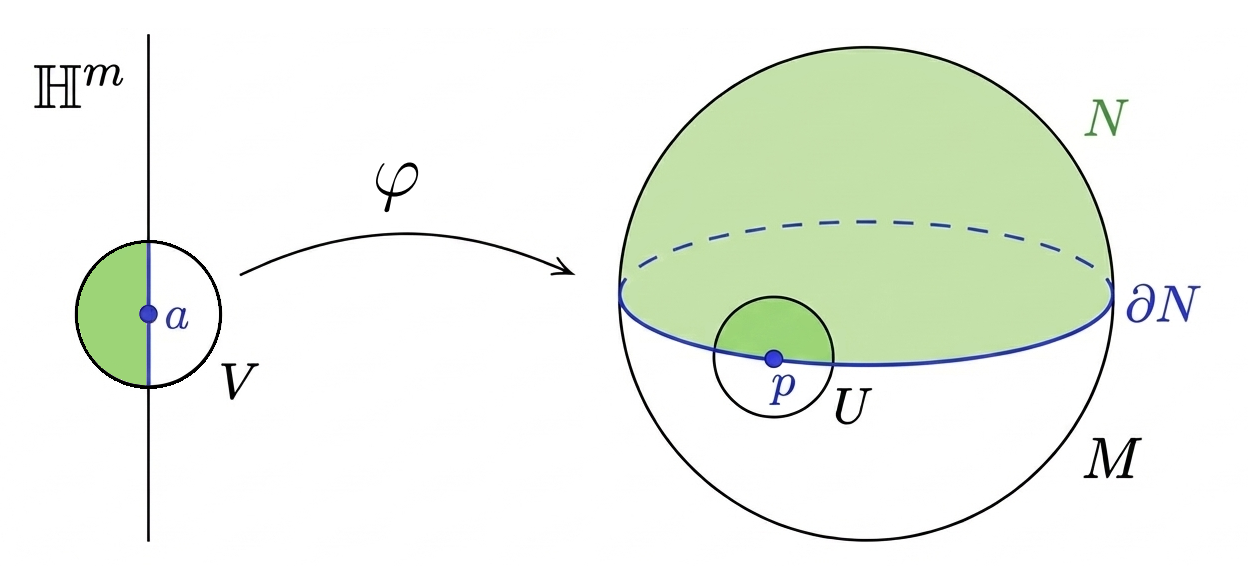
\includegraphics[width=0.5\textwidth, ]{Pictures/edge.png}
		\caption{\raggedright Иллюстрация к определению регулярной области.}
		\label{fig:edge}
\end{framed}
\vspace{-15pt}
\end{figure}
\end{definition}



\begin{note}
    По критерию непрерывности гомеоморфизм отображает открытые множества в открытые. Поэтому параметризация $\phi$ переводит внутренние (внешние) точки $V \cap \mathbb{H}^m$ во внутренние (внешние) точки $U \cap N$, а значит, $\phi(V \cap \partial \mathbb{H}^m) = U \cap \partial N$.
\end{note}

\begin{lemma}
    Пусть $M$ -- гладкое $m$-мерное многообразие, $N$ -- регулярная область в $M$. Тогда $\partial N$ является гладким $(m-1)$-мерным многообразием.
\end{lemma}

\begin{myproof}
	Пусть $p \in \partial N$, $\phi : V \to U$ -- параметризация окрестности $p$ в $M$ из определения $N$.
    Отождествим $\R^{m-1}$ и $\partial \mathbb{H}^m$ по правилу $L(x') = (0, x')$.
	Рассмотрим $V_0 \subset \R^{m-1}$ такое, что $\{0\} \times V_0 = V \cap \partial \mathbb{H}^m$ и обозначим $U_0 = U \cap \partial N$.
	Тогда $V_0$ открыто в $\R^{m-1}$ как сечение открытого множества и $\phi_0: V_0 \to U_0$, заданное как $\phi_0 = \phi \circ L$, есть параметризация $\partial N$.
	Действительно, $\phi_0$ гладкое в силу гладкости $\phi$, матрица $D\phi_0$ получается из $D\phi$ вычеркиванием первого столбца, поэтому ранг новой матрицы максимален, и отображение $\phi_0$ является гомеоморфизмом как сужение гомеоморфизма $\phi$ на $\{x_1 = 0\}$. % непрерывно как сужение $\phi^{-1}|_{U_0}$.
\end{myproof}

\begin{definition}
	Многообразие $\partial N$ называется \textit{краем} $N$.
\end{definition}

Следующее утверждение дает важнейший источник регулярных областей.

\begin{theorem}
    Пусть $M$ -- гладкое $m$-мерное многообразие, $u \ f: M \to \R$ -- гладкая функция, такая что $f^{-1}(0) \ne \emptyset$ и $df_p \ne 0$ для всех $p \in f^{-1}(0)$. Тогда
    \[
    B := f^{-1}(-\infty, 0) = \{p \in M : f(p) < 0\}
    \]
    является регулярной областью с краем $\partial B = f^{-1}(0)$.
\end{theorem}

\begin{myproof}
    Множество $B$ открыто в $M$ как прообраз открытого луча при непрерывном отображении.
    % Найдем такую параметризацию, что координатное представление $f$ относительно этой параметризации является проекцией на первую координату.
    Пусть $p \in \partial B$, тогда $p \in f^{-1}(0)$ из непрерывности. Выберем параметризацию $\phi: V \to U$ окрестности $p$ в $M$ и рассмотрим $g = f \circ \phi$. Если $p = \phi(a)$, то $dg_a = df_p \circ d\phi_a$, так что $dg_a \ne 0$. Заменяя координаты, можно считать, что $\frac{\partial g}{\partial x_1}(a) \ne 0$.
    Рассмотрим на $V$ функцию $F(x) = (g(x), x_2, \dots, x_m)$. Матрица Якоби $DF = \begin{pmatrix} \frac{\partial g}{\partial x_1} & \frac{\partial g}{\partial x_2} \dots \frac{\partial g}{\partial x_m} \\ 0 & E_{m-1} \end{pmatrix}$, поэтому $\det DF(a) \ne 0$. Тогда по теореме об обратной функции найдутся открытые в $\R^m$ множества $W$ и $V_0$, $a \in V_0 \subset V$, что сужение $F: V_0 \to W$ является диффеоморфизмом.
    Положим $U_0 = \phi(V_0)$, $\psi = \phi \circ F^{-1}$. Тогда $\psi$ -- параметризация окрестности $p$ в $M$ и на $W$ имеем:
    \[
    f \circ \psi(x) = f \circ \phi \circ F^{-1}(x) = g(F^{-1}(x_1, \dots, x_m)) = x_1,
    \]
    Следовательно, $\psi(W \cap \mathbb{H}^m) = \psi\{x \in W : x_1 < 0\} = B \cap U_0$. Кроме того, для $p \in f^{-1}(0)$ верно $x_1 = 0$ ($\psi(x) = p$), откуда $p \in \partial B$ по замечанию выше и утверждение доказано.
\end{myproof}

\begin{corollary}
    Шар $B^m = \{x \in \R^m : |x| < 1\}$ есть регулярная область с краем $\partial B^m = S^{m-1}$.
\end{corollary}

\begin{myproof}
    Действительно, положим гладкую функцию $f(x) = |x|^2 - 1$. Тогда $B^m = f^{-1}(-\infty, 0)$ и $\rk df_p = 1$ для всех $p \in f^{-1}(0) = S^{m-1}$.
	По теореме заключаем требуемое.
\end{myproof}


\subsection{Ориентация гладких многообразий}

\begin{definition}
    Пусть $M$ -- гладкое многообразие.
    \begin{enumerate}[itemsep = 0pt, topsep = 5pt]
		\item Семейство параметризаций $\mathcal{A} = \{\phi_\alpha: V_\alpha \to U_\alpha, \ \alpha \in I\}$, образы которых покрывают $M$, называется \textit{атласом} на $M$.
		\item Атлас на $M$ называется \textit{ориентирующим}, если якобианы всех его функций перехода положительны.
		\item Гладкое многообразие, на котором задан ориентирующий атлас, называется \textit{ориентированным}.
		\item Если на гладком многообразии существует ориентирующий атлас, то оно называется \textit{ориентируемым}.
		\item Ориентация многообразия -- класс эквивалентности ориентирующих атласов, где два атласа эквивалентны, если их объединение является ориентирующим атласом.
	\end{enumerate}
\end{definition}

\begin{example}
    Любое непустое открытое подмножество $\R^m$ ориентируемо. Его ориентирующий атлас состоит из тождественной параметризации.
\end{example}

\begin{problem}
    Гладкое 2-мерное многообразие в $\R^3$ ориентируемо тогда и только тогда, когда на нем существует непрерывное поле единичных нормалей.
\end{problem}

\begin{note}
	Существуют неориентируемые многообразия. 
	Без доказательства отметим, что лист Мёбиуса не является ориентируемым двумерным многообразием в $\R^3$.
\end{note}

\begin{note}
    Пусть на $M$ при помощи атласа $\mathcal{A}$ задана ориентация.
	Рассмотрим параметризацию $\phi: V \to U$ на $M$, где $U$ связно.
	Если $\phi$ \textit{не соответствует ориентации $M$}, то есть $\mathcal{A} \cup \{\phi\}$ не является ориентирующим, то параметризация $\phi \circ A$, где $A(x_1, \dotsc, x_m) = (x_1, \dotsc, -x_m)$ уже соответствует ориентации $M$.
	Действительно, ранее якобиан перехода от любой карты $\psi \in \mathcal{A}$ к $\phi$ был отрицателен, а теперь станет положителен. 
\end{note}

\begin{theorem}
    Пусть $M$ -- гладкое $m$-мерное ориентируемое многообразие ($m > 1$), $N$ -- регулярная область в $M$. Тогда многообразие $\partial N$ также ориентируемо.
\end{theorem}

\begin{myproof}
    По определению $\partial N$ покрывается образами параметризаций $\phi$ с условием $\phi(V \cap \mathbb{H}^m) = U \cap N$. Из предыдущего замечания следует, что каждую из таких параметризаций можно считать соответствующей ориентации $M$.
	Пусть $\phi$ и $\psi$ -- такие параметризации на $M$ в окрестности $p \in \partial N$. Покажем, что если функция перехода между $\phi$ и $\psi$ имеет положительный якобиан, то это же выполнено и для $\phi_0$ и $\psi_0$ в терминологии из леммы 8.1.
    Пусть $\Phi = \psi^{-1} \circ \phi$ ($\det D \Phi > 0$), $\Phi = (\Phi_1, \dots, \Phi_m)$ и $\Phi_0 = \psi_0^{-1} \circ \phi_0$. Тогда $\Phi_0 = (\Phi_2 \circ L, \dots, \Phi_m \circ L)$. Если $\phi(0, a) = p$, то $\Phi(0, a) = (0, \Phi_0(a))$ и это же верно и для точек, близких к $a$. Значит, $\frac{\partial \Phi_1}{\partial x_i}(0, a) = 0$ для $i \geq 2$. Поэтому
    \[
    D\Phi(0, a) = \begin{pmatrix} \frac{\partial \Phi_1}{\partial x_1}(0, a) & 0 \dots 0 \\ * & D\Phi_0(a) \end{pmatrix}.
    \]
    Следовательно, $\det D\Phi(0, a) = \frac{\partial \Phi_1}{\partial x_1}(0, a) \det D\Phi_0(a)$.
	Поскольку $\Phi$ отображает $\mathbb{H}^m$ в себя ($\Phi_1 < 0$ для точек из $\mathbb{H}^m$), то $\frac{\partial \Phi_1}{\partial x_1}(0, a) = \lim \limits_{t \to -0} \frac{1}{t}(\Phi_1(t, a) - 0) \ge 0$. 
	Равенство нулю невозможно, так как $\det D\Phi(0, a) > 0$. Заключаем, что $\det D\Phi_0(a) > 0$, что и требовалось.
\end{myproof}

\begin{note}
	Таким образом, заданная ориентация $M$ индуцирует ориентации на $N$ и на $\partial N$: надо сузить параметризации из ориентации $M$ на $N$ (как на открытое множество) и на $\partial N$ (в смысле леммы 8.1) соответственно. Полученные ориентации $N$ и его края $\partial N$ будем называть \textit{согласованными}.
\end{note}

\begin{lemma}
    Пусть гладкое $m$-мерное многообразие $M$ в $\R^{m+1}$ задано уравнением, то есть $M = f^{-1}(0)$, где функция $f: U \subset \R^{m+1} \to \R$ -- гладкая с $\rk df_p = 1$ для всех $p \in M \cap U$. Тогда $M$ ориентируемо.
\end{lemma}

\begin{myproof}
    По теореме 8.1 имеем $M = \partial B$, где $B = \{p \in \R^{m+1}: f(p) < 0\}$. Так как многообразие $B$ ориентируемо как открытое множество, то $M = \partial B$ ориентируемо по теореме 8.2.
\end{myproof}

\begin{example}
    Сфера $S^m$ -- ориентируемое гладкое многообразие.
\end{example}
